% ============================================================================
% Utah AI Convergence 2026 --- Advanced Manufacturing Academic Panel
% 10-minute talk: Autonomous alloy discovery via additive manufacturing
% Presenter: Sterling G. Baird (BYU Mechanical Engineering)
%
% Design follows Jean-luc Doumont's "Trees, maps, and theorems" principles:
%   * one message per slide, stated as a full-sentence "message title"
%   * slides carry the minimum the audience must SEE; the rest is spoken
%   * speaker-oriented detail lives in \note{...}, never on the slide
%
% BUILD (see Makefile):
%   make slides   -> talk.pdf            (audience deck, no notes)
%   make notes    -> talk-notes.pdf      (deck + speaker notes, for rehearsal)
%   make handout  -> talk-handout.pdf    (one frame per page, overlays collapsed)
% Toggle is set at build time via \def\shownotes{} / \def\handout{}; do not
% edit the \setbeameroption lines by hand.
% ============================================================================
\ifdefined\handout
  \documentclass[handout,aspectratio=169,11pt]{beamer}
\else
  \documentclass[aspectratio=169,11pt]{beamer}
\fi

% --- Theme: plain and uncluttered (Doumont: remove non-signal ink) ----------
\usetheme{default}
\usecolortheme{seagull}
\setbeamertemplate{navigation symbols}{}     % drop navigation clutter
\setbeamertemplate{footline}[frame number]
\setbeamertemplate{itemize items}[circle]
\setbeamerfont{frametitle}{size=\large,series=\bfseries}
\setbeamercolor{frametitle}{fg=black}
\setbeamercolor{structure}{fg=black!80}

% --- Speaker notes: shown only in the notes build ---------------------------
\usepackage{pgfpages}
\ifdefined\shownotes
  \setbeameroption{show notes}
  \setbeamertemplate{note page}{%
    \insertnote\par}
\fi

\usepackage[T1]{fontenc}
\usepackage{lmodern}
\usepackage{booktabs}
\usepackage{tikz}
\usetikzlibrary{arrows.meta,positioning}

% --- A few shorthands --------------------------------------------------------
\newcommand{\flaime}{\textsc{Flaime}}
\definecolor{accent}{RGB}{160,0,0}        % matches the convergence red
\newcommand{\msg}[1]{\textbf{#1}}

\title{Closing the loop on aerospace alloys}
\subtitle{Autonomous discovery via additive manufacturing}
\author{Sterling G.\ Baird}
\institute{Vertical Cloud Lab \,$\cdot$\, Mechanical Engineering, BYU}
\date{Utah AI Convergence 2026 \,$\cdot$\, Advanced Manufacturing Panel}

\begin{document}

% ----------------------------------------------------------------------------
\begin{frame}[plain]
  \titlepage
\end{frame}
\note{%
  Sterling Baird, BYU. Ten minutes, one idea: run the alloy-development loop
  automatically and overnight --- the way software teams run automated builds and
  tests --- and the computing tools that make that work transfer to almost any
  manufacturing sector. Allotment: ~2 min on the problem, ~4 min on closing the
  loop, ~3 min on the transferable tools, ~1 min margin. Acknowledge the
  organizers and Ashley Spear for the panel invite.}

% ----------------------------------------------------------------------------
\begin{frame}{We import the elements our best alloys depend on}
  \begin{columns}[T]
    \begin{column}{0.52\textwidth}
      \begin{itemize}
        \item \textbf{100\%} of manganese --- imported
        \item \textbf{100\%} of zirconium concentrates --- imported
        \item \textbf{74\%} of chromium --- imported
      \end{itemize}
      \vspace{1em}
      These are the workhorses of high-performance aluminum alloys
      for additive manufacturing.
    \end{column}
    \begin{column}{0.44\textwidth}
      \begin{block}{The exposure}
        One supply disruption can idle a domestic AM production line.
      \end{block}
    \end{column}
  \end{columns}
\end{frame}
\note{%
  Source: USGS 2024. The point isn't the exact numbers --- it's that our highest
  performing structural aluminum alloys are built on elements we don't control.
  A single supply shock idles the printers. So there are really two goals at
  once: find high-performing alloys AND reduce how much critical mineral they
  need. That "dual mandate" is exactly the DOE Genesis Mission Topic 3B framing
  we're pursuing.}

% ----------------------------------------------------------------------------
\begin{frame}{The bottleneck is the development loop, not the printer}
  \begin{center}
  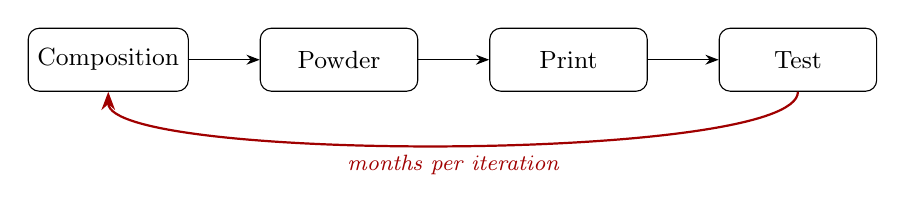
\begin{tikzpicture}[node distance=7mm and 9mm,
      box/.style={draw,rounded corners,minimum height=8mm,minimum width=20mm,
                  font=\small,align=center},
      >=Stealth]
    \node[box] (c) {Composition};
    \node[box,right=of c] (p) {Powder};
    \node[box,right=of p] (pr){Print};
    \node[box,right=of pr](t) {Test};
    \draw[->] (c)--(p); \draw[->] (p)--(pr); \draw[->] (pr)--(t);
    \draw[->,accent,thick] (t.south) .. controls +(0,-9mm) and +(0,-9mm) ..
      node[below,font=\footnotesize\itshape]{months per iteration} (c.south);
  \end{tikzpicture}
  \end{center}
  \vspace{0.5em}
  \begin{center}
  Each turn of the loop is slow, manual, and run \emph{one alloy at a time}.
  \end{center}
\end{frame}
\note{%
  Traditional alloy development is a hand-cranked loop: pick a composition, make
  powder, print specimens, test them, then a human decides what to try next ---
  and that cycle is months long, run sequentially. That's why a new aerospace
  alloy can take a decade-plus and millions of dollars. The expensive resource
  isn't compute, it's wall-clock iterations. Everything that follows is about
  spending fewer, smarter iterations.}

% ----------------------------------------------------------------------------
\begin{frame}{AI can drive the whole pipeline, stage by stage}
  \begin{center}
  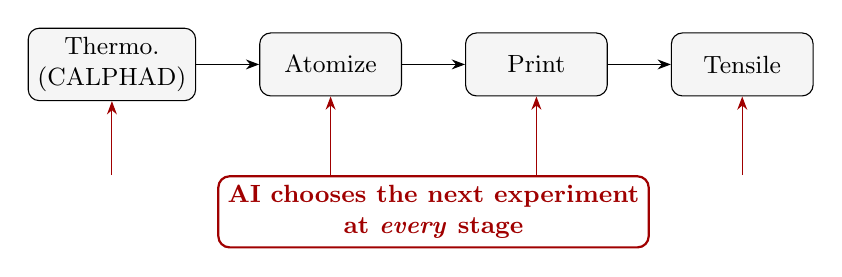
\begin{tikzpicture}[node distance=6mm and 8mm,
      stage/.style={draw,rounded corners,fill=black!4,minimum height=8mm,
                    minimum width=18mm,font=\small,align=center},
      brain/.style={draw,accent,thick,rounded corners,minimum width=30mm,
                    font=\small\bfseries,align=center},
      >=Stealth]
    \node[stage] (s1){Thermo.\\(CALPHAD)};
    \node[stage,right=of s1](s2){Atomize};
    \node[stage,right=of s2](s3){Print};
    \node[stage,right=of s3](s4){Tensile};
    \draw[->](s1)--(s2);\draw[->](s2)--(s3);\draw[->](s3)--(s4);
    \node[brain,below=10mm of s2.south east,xshift=4mm] (b)
      {AI chooses the next experiment\\ at \emph{every} stage};
    \draw[->,accent](b.north-|s1)--(s1.south);
    \draw[->,accent](b.north-|s2)--(s2.south);
    \draw[->,accent](b.north-|s3)--(s3.south);
    \draw[->,accent](b.north-|s4)--(s4.south);
  \end{tikzpicture}
  \end{center}
  \vspace{0.3em}
  \begin{center}
  Model each stage as a node; optimize the workflow end-to-end, cost-aware.
  \end{center}
\end{frame}
\note{%
  Instead of optimizing the final property in isolation, we model each
  manufacturing stage --- thermodynamics, atomization, printing, testing --- as a
  node in a function network (a directed acyclic graph). The method is Bayesian
  Optimization over Function Networks, BOFN, with a partial-knowledge-gradient
  acquisition function. In plain terms: the AI can stop a bad candidate after a
  cheap CALPHAD check instead of paying to print and test it. It picks the most
  informative experiment at each stage, accounting for how much that experiment
  costs. Don't read the acronyms aloud --- just say "it decides, stage by stage,
  what's worth doing next."}

% ----------------------------------------------------------------------------
\begin{frame}{\flaime: same loop, run automatically overnight}
  \begin{columns}[T]
    \begin{column}{0.5\textwidth}
      \textbf{Screen in silico, in parallel}
      \begin{itemize}
        \item \(\sim\)23{,}000 element combinations
        \item thermodynamics + solidification, run in parallel
      \end{itemize}
      \vspace{0.6em}
      \textbf{Validate the few that survive}
      \begin{itemize}
        \item top 3--6 systems, 100--200 compositions
        \item powder $\to$ print $\to$ tensile
      \end{itemize}
    \end{column}
    \begin{column}{0.5\textwidth}
      \begin{block}{Phase~I target (not yet measured)}
        Aim: \(\sim\)\textbf{10\(\times\)} faster
        powder-to-property\\[2pt]
        \footnotesize(planning estimate: \(\sim\)3\(\times\) smarter selection
        \(\times\) \(\sim\)3\(\times\) closed-loop execution)
      \end{block}
      \begin{block}{Phase~I goal}
        Concept $\to$ lab-validated closed loop.
      \end{block}
    \end{column}
  \end{columns}
\end{frame}
\note{%
  This is the project, FLAIME, "Fast Learning AI for Mineral Efficiency." The
  shape: explore tens of thousands of compositions cheaply and in parallel on
  HPC, then spend real powder and printer time only on the handful that survive.
  Roughly 3x from AI choosing better experiments, times another ~3x from running
  the loop closed instead of by hand, gives an order-of-magnitude target. Numbers
  are targets, not yet results --- Phase I is about validating the closed loop on
  real aluminum alloys, moving from concept (TRL 2) to lab-validated (TRL 4).
  Software-orchestrated with human operators now; architected for robots next.}

% ----------------------------------------------------------------------------
\begin{frame}{These tools transfer to any staged manufacturing workflow}
  \begin{columns}[T]
    \begin{column}{0.5\textwidth}
      \begin{block}{Start optimization without custom code}
        \textsc{Honegumi} generates a runnable optimization
        template from a few toggles.
      \end{block}
      \begin{block}{Use cheap screens before expensive tests}
        Stage-aware optimization kills bad candidates early.
      \end{block}
    \end{column}
    \begin{column}{0.5\textwidth}
      \begin{block}{Prototype automation on cheap stand-ins}
        Frugal twins de-risk capital purchases before you buy
        the expensive machine.
      \end{block}
      \begin{block}{Make experiments shareable and reproducible}
        Cloud execution plus open, reusable (FAIR) data and models.
      \end{block}
    \end{column}
  \end{columns}
\end{frame}
\note{%
  This is the slide the organizers asked for --- what's useful outside alloys.
  (1) Honegumi: our open template engine, "skeletal framework" in Japanese ---
  pip install honegumi --- it generates a correct, runnable Bayesian-optimization
  script from a click grid, so a process engineer doesn't have to be a BO expert.
  (2) The function-network framing: any multi-step process --- semiconductors,
  composites, food, pharma --- can be modeled stage-by-stage and optimized
  cost-aware. (3) Frugal twins: cheap hardware twins to prototype automation at
  low risk before capital spend. (4) Cloud experimentation plus FAIR data: remote
  access and shareable data/models. The takeaway: these are
  domain-agnostic. Point interested attendees to the GitHub organization and
  Honegumi docs.}

% ----------------------------------------------------------------------------
\begin{frame}[plain]
  \vfill
  \begin{center}
    {\Large\textbf{Run the loop like software: automate it, share it.}}\\[1em]
    {\normalsize Sterling Baird \,$\cdot$\, \texttt{github.com/vertical-cloud-lab}}\\
    {\footnotesize Honegumi: \texttt{honegumi.readthedocs.io} \,$\cdot$\,
      \texttt{pip install honegumi}}
  \end{center}
  \vfill
\end{frame}
\note{%
  Close on the one-liner: treat the manufacturing development loop like a
  software pipeline --- automate the iterations, share the data and the tooling.
  Point to the lab org and Honegumi. Then hand back to the moderator / open for
  panel questions. Watch the clock: if short on time, cut the FLAIME numbers
  slide detail, not the transferable-tools slide.}

\end{document}
